\documentclass[12pt]{article}
\title{Project Report \#2}
\author{Andre Sealy, Federica Malamisura, Swapnil Pant}
\usepackage{amsmath, amsfonts, amssymb, amsthm,}
\usepackage{tikz}
\usetikzlibrary{matrix,positioning}
\tikzset{bullet/.style={circle,fill,inner sep=2pt}}
\usepackage{braket}
\usepackage{bbold}
\usepackage[margin=1.0in]{geometry}
\usepackage{mathtools}
\usepackage{xfrac}
\usepackage{xcolor}
\newcommand{\lam}{$\lambda$}
\usepackage{pgfplots}
\tikzset{My Style/.style={samples=100, thick}}
\usepackage{graphicx}
\usepackage{pgfplots}
\usepackage{setspace}
\usepackage{enumerate}
\usepackage{hyperref}
\usepackage{array}
\usepackage{listings}
\usepackage[official]{eurosym}
\usepackage[shortlabels]{enumitem}
\usepackage{booktabs}
\usepackage{floatrow}
\usepackage{listings}
\floatsetup[table]{capposition=top}
\usepackage{appendix}
\usepackage{xcolor}
\hypersetup{
	colorlinks,
	linkcolor={red!50!black},
	citecolor={blue!50!black},
	urlcolor={blue!80!black}
}
% Set the overall layout of the tree
\tikzstyle{level 1}=[level distance=4.5cm, sibling distance=4.5cm]
\tikzstyle{level 2}=[level distance=3.5cm, sibling distance=2cm]

% Define styles for bags and leafs
\tikzstyle{bag} = [text width=5em, text centered]
\tikzstyle{end} = [circle, minimum width=3pt,fill, inner sep=0pt]

\makeatletter
\def\amsbb{\use@mathgroup \M@U \symAMSb}
\makeatother

\lstdefinestyle{mystyle}{
	backgroundcolor=\color{backcolour},   
	commentstyle=\color{codegreen},
	keywordstyle=\color{magenta},
	numberstyle=\tiny\color{codegray},
	stringstyle=\color{codepurple},
	basicstyle=\ttfamily\footnotesize,
	breakatwhitespace=false,         
	breaklines=true,                 
	captionpos=b,                    
	keepspaces=true,                 
	numbers=left,                    
	numbersep=5pt,                  
	showspaces=false,                
	showstringspaces=false,
	showtabs=false,                  
	tabsize=2
}
\onehalfspacing

\begin{document}

\maketitle

\section{Overview of the Asset and the Market}

The asset class for our time series analysis consists of equities primarily in the Technology sector. The reason for choosing the technology sector out of many industry classifications is multifaceted and involves numerous foundational considerations. First, we consider that tech stocks often have higher betas (meaning, they move with the market) on average, suggesting higher annualized volatility. Second, they are more sensitive to new information related to innovation cycles, such as new product releases, software updates, and research. Finally, we have the growth aspect, which involves the shifts in macroeconomic trends (such as interest rates), global demand, and supply chains. The border macroeconomic environment and the fundamentals make tech stocks an ideal candidate for time series analysis.

\section{Properties of the Time-Series}

In this section, we will outline foundational descriptive statistics, which involve the statistical moments and distributions of our sample securities and time series analysis.

\subsection{Descriptive statistics}
First, we outline a few sample statistics for the stocks in our sample. These statistics involves the sample mean, denoted by
\begin{equation}
	\hat{\mu}_x=\frac{1}{T}\sum_{t=1}^{T}x_t,
\end{equation}
the sample standard deviation, denoted by,
\begin{equation}
	\hat{\sigma}_x=\sqrt{\frac{1}{T-1}\sum_{t=1}^{T}\left(x_t-\hat{\mu}_2\right)^2},
\end{equation}
the sample skewness, denoted by
\begin{equation}
	\hat{S}(x)=\frac{1}{\left(T-1\right)\hat{\sigma}^3_x}\sum_{t=1}^{T}\left(x_t-\hat{\mu}_x\right)^3,
\end{equation}
and the sample kurtosis (excess kurtosis), denoted by
\begin{equation}
	\hat{K}(x)=\frac{1}{\left(T-1\right)\hat{\sigma}^4_x}\sum_{t=1}^{T}\left(x_t-\hat{\sigma}_x\right)^4.
\end{equation}
The sample mean, $\hat{\mu}_x$ represents the daily average simple (or log) returns, where $T$ are the number of days in the sample. The sample standard deviation, denoted by $\hat{\sigma}_x$, represents the daily realized volatility, the universal risk measurement. Table (\ref{tab:descriptive}) shows the descriptive statistics of the tech stocks in our sample of the daily sample returns. The start date of our analysis is January 3rd, 2007, which gives us a time interval of roughly 18 years. In addition to the sample mean, standard deviation, skewness, and excess kurtosis, we have also decided to include the minimum and maximum prices within this time period for a better perspective.
\begin{table}[ht]
	\centering
	\caption{Descriptive statistics of Tech Stocks (\textit{Daily Simple Returns \%})}
	\begin{tabular}[t]{lcccccc}
		\toprule
		Security & Mean ($\hat{\mu}_x$) & Std Dev ($\hat{\sigma}_x$) & Skewness ($\hat{S}(x)$) & Kurtosis ($\hat{K}(x)$) &Min&Max \\
		\midrule
		QCOM & 0.05 & 2.17 & 0.27 & 9.53 &-15.25&23.20 \\
		\bottomrule
	\end{tabular}\label{tab:descriptive}
\end{table}

The returns between our sample securities are roughly similar when we look at daily log returns in Table (\ref{tab:log_descriptiv}).

The sample skewness measures the asymmetry of a probability distribution around the sample mean. It helps determine whether our sample is skewed more towards one side of the distribution. If the sample skewness, $\hat{S}(x)\approx 0,$ the distribution is symmetrical. Based on skewness, QCOM, CSCO is roughly symmetrical, as the skewness is approximately 0. 
\begin{table}[ht]
	\centering
	\caption{Descriptive statistics of Tech Stocks (\textit{Daily Log Returns \%})}
	\begin{tabular}[t]{lcccccc}
		\toprule
		Security & Mean ($\hat{\mu}_x$) & Std Dev ($\hat{\sigma}_x$) & Skewness ($\hat{S}(x)$) & Kurtosis ($\hat{K}(x)$) &Min&Max \\
		\midrule
		QCOM & 0.21 & 1.06 &-1.53 & 5.03 &-16.54 &3.18 \\	
		\bottomrule
	\end{tabular}\label{tab:log_descriptiv}
\end{table}
On the hand, the sample kurtosis measures how heavy the tails of the probability distribution are, which helps assess the presence of extreme values and the frequency of their occurrence. A normal distribution has a sample kurtosis of  $\hat{K}(x)\approx 3$, which indicates a normal distribution. All of the securities in our sample have extremely high kurtosis, which is natural for equities, considering financial markets experience extreme price movements more frequently than a normal distribution would predict. Financial markets also show periods of high and low volatility; when volatility spikes, returns tend to have more extreme values.

Considering the sample skewness, AMD is much further away from 0. There is some slight positive skew QCOM. We do not have a single sample statistic that we can use to differentiate skewed versus unskewed. However, we can test for skewness using the Jarque and Bera test for normality.

The Jarque-Bera (JB) test is a statistical test used to check whether a dataset follows a normal distribution. It does this by examining the skewness and kurtosis of the dataset with the following formula:
\begin{equation}
	JB= \underbrace{\frac{\hat{S}^2(r)}{\sqrt{\sfrac{6}{T}}}}_{\textit{skewness}}  +\overbrace{\frac{[\hat{K}(r)-3]^2}{\sfrac{24}{T}}}^{\textit{kurtosis}}
\end{equation}
which is distributed as a chi-square, $\mathcal{X}^2$, random variable with 2 degrees of freedom. Given the sample of returns, $\lbrace r_1,\ldots,r_T\rbrace$, to test the skewness of the returns, we consider the following hypothesis test
\[
\begin{aligned}
	H_0&:S(r)= 0\\
	H_a&:S(r)\neq 0\\
\end{aligned}
\]
where the $t-$statistic is 
\begin{equation}
	t=\frac{\hat{S}(r)}{\sqrt{\sfrac{6}{T}}}
\end{equation}
We would also need to conduct a hypothesis test for the excess kurtosis, which is
\[
\begin{aligned}
	H_0&:K(r)-3= 0\\
	H_a&:K(r)-3\neq 0\\
\end{aligned}
\]
where the $t-$statistics is the following:
\begin{equation}
	t=\frac{\hat{K}(r-3)}{\sqrt{\sfrac{24}{T}}}
\end{equation}
We provide the JB-test for statistical normality with the skewness, $\hat{S}(x)$, kurtosis, $\hat{K}(x)$, t-statistic, $\mathcal{X}^2$, and p-values. We reject the null-hypothesis, $H_0$ of normality if the $p-$value of the JB statistic is less than the significance level. As the Table (\ref*{tab:jbtest}) shows, the $p$-values of the JB-test for our sample securities are significantly below the 5\% significance level, which indicates that MSFT, QCOM, AMD are skewed to the right (positively skewed) and ADBE are negatively skewed.
\begin{table}[ht]
	\centering
	\caption{Jarque-Bera Statistical Test for Normality for log daily returns}
	\begin{tabular}[t]{lcccc}
		\toprule
		Security & Skewness ($\hat{S}(x)$) & Kurtosis ($\hat{K}(x)$) & $t$-statistic ($\mathcal{X}^2$) & $p$-value \\
		\midrule
		QCOM & 0.27 & 9.53 & 14733.69 & 2.2e-16 \\				
		\bottomrule
	\end{tabular}\label{tab:jbtest}
\end{table}

\subsection{Visualization}
We first begin our analysis by looking at cumulative returns, an essential part of time series analysis. Unlike daily or periodic returns, which can be volatile, cumulative returns smooth out fluctuations and show the overall trends of a time series. They also help compare the growth of our asset class over different time horizons and identify long-term trends in the market. Cumulative returns will serve as the basis for other predicting and forecasting techniques.
\begin{figure}[h]
	\centering
	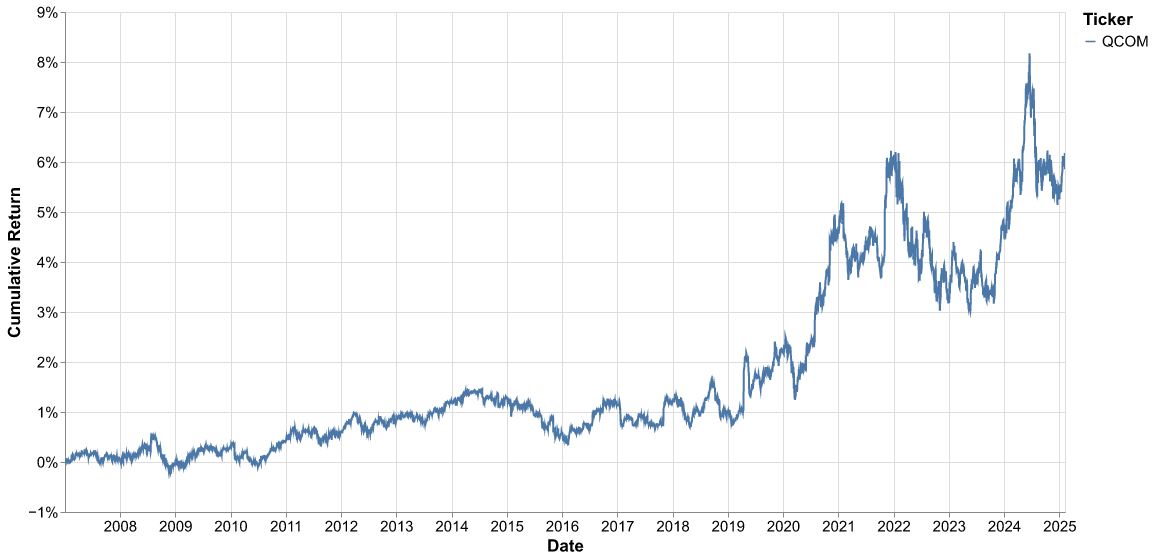
\includegraphics[width=0.9\linewidth]{plots/cumulative_returns_qcom}
	\caption{Cumulative Returns for the sample securities}
	\label{fig:cum_returns}
\end{figure}
Figure (\ref{fig:cum_returns}) shows the cumulative returns for QCOM. Cumulative returns ignore risk and measure the total percentage return, whereas metrics such as the standard deviation, $\hat{\sigma}_x$, and kurtosis, $\hat{K}(x)$, account for risk. The idea of studying volatility is that the returns of our asset $\lbrace r_t\rbrace$ have a serial correlation, or it may merely be stationary. The Autocorrelation Function (ACF) measures the correlation between a time series and its own past values at different lags. It helps identify patterns, dependencies, and stationarity in time series data. When considering a weakly stationary return series, $r_t$, the linear dependence between $r_t$ and past values of $t_{t-i}$ is called the lag-$\ell$ autocorrelation of $r_t$, denoted by the following:
\begin{equation}
	\hat{\rho}_\ell=\frac{\sum_{t=\ell+1}^{T}\left(r_t-\bar{r}\right)\left(r_{t-\ell}-\bar{r}\right)}{\sum_{t=1}^{T}\left(r_t-\bar{r}\right)^2},\quad 0\leq\ell<T-1
\end{equation}
For testing several autocorrelations jointly, we have the Ljung and Box test, denoted by,
\begin{equation}
	\mathcal{Q}(m)=T(T+2)\sum_{\ell=1}^{m}\frac{\hat{\rho}_\ell^2}{T-\ell}
\end{equation}
The hypothesis test for Ljung and Box is established as follows:
\[
\begin{aligned}
	H_0&:\rho_1=\cdots=\rho_m=0\\
	H_a&:\rho_i\neq 0
\end{aligned}
\]
for some $i\in\lbrace1,\ldots,m\rbrace$. We assume that $\lbrace r_t\rbrace$ is an iid sequence and $\mathcal{Q}^*(m)$ is a chi-squared random variable, $\mathcal{X}$, with $m$ degrees of freedom. The decision rule is to reject $H_0$ if $\mathcal{Q}(m)>\mathcal{X}^2_\alpha$, where $\mathcal{X}^2_\alpha$ denotes the $100\left(1-\alpha\right)$th percentile of a chi-squared distribution. 

Figure (\ref{fig:acf_plot}) shows the sample autocorrelation functions of the monthly log returns from January 2007 to November 2025. We have used a maximum of 20 lags. In each plot, two horizontal dashed lines denote two standard error limits of ACF. The sample ACFs or the MSFT plot are very close to each other, and they suggest that the serial correlations of monthly MSFT log stock returns are very small, if any. The sample ACFs are all within their two standard error limits, indicating that they are not significantly different from zero at the 5\% level.

\begin{figure}[h]
	\centering
	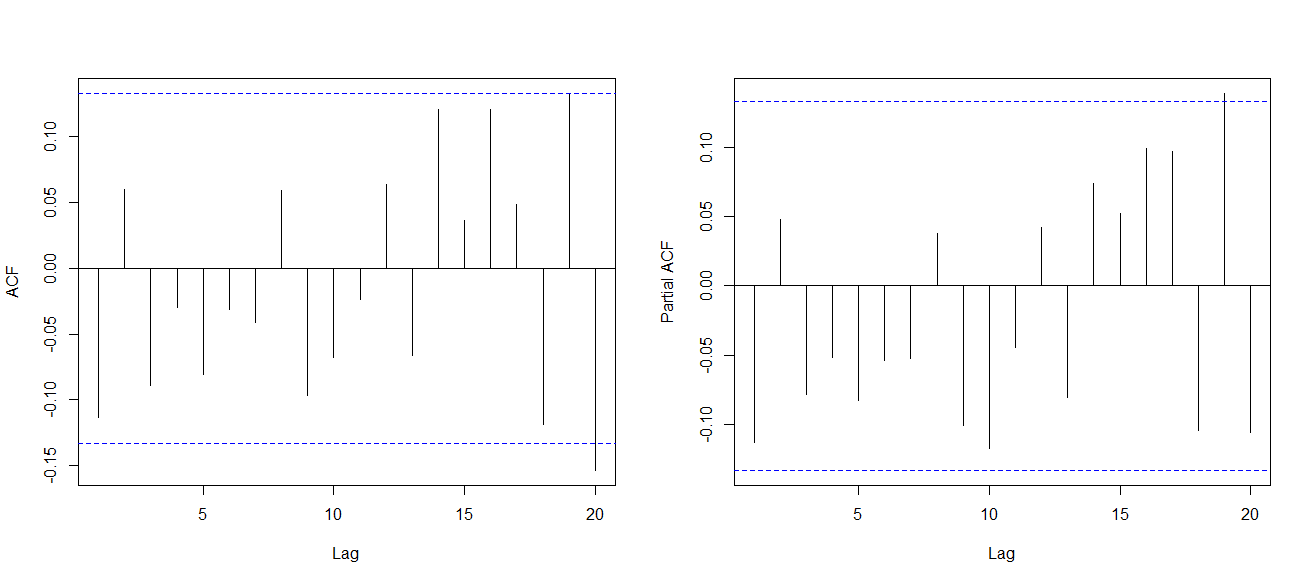
\includegraphics[width=0.9\linewidth]{plots/qcom_acf_pacf.png}
	\caption{ACF and PACF of QCOM}
	\label{fig:qcom_acf_pacf}
\end{figure}

Regarding the log monthly returns for the other securities in our sample, we find there is at least one lag that determines a significant serial correlation with previous returns. For QCOM, this occurs at lag 17, From looking at the ACF plots, it would appear that these lags barely reach the rejection threshold of 2 times the standard error. However, we can perform the Ljung-Box statistic determine if there are some significant serial correlations at the 5\% level for all return series. The Ljung-Box statistic with the max lag gives us a p-value of 0, so we reject the null-hypothesis.

As we can see from the test statistics and the $p$-values, the only securities with a significant serial correlation with monthly log returns are QCOM. What we can interpret from this data, at least for long monthly returns, is that there is no significant serial correlation. It may be worth using a more frequent observation series, such as daily.

We have also looked at the Partial Autocorrelation Function (PACF) of the log monthly returns. The PACF is used to directly measure the relationship between a time series and its past values at different lags while removing the influence of the intermediate lags. Unlike the ACF, which includes direct and indirect correlations, the PACF isolates the pure effect of each lag on the present value.

Figure (\ref{fig:pacf_plot})shows the PACF for the log monthly returns for our sample securities. We have used a maximum of 20 lags. After accounting for intermediate lags, each bar in the PACF plot represents the correlation between the time series and its lagged version. The dashed lines represent the 95\% confidence interval. Any bar extending beyond these lines is statistically significant. ADBE and CSCO all appear to have significant lags.

ADBE have significant lags at month 6 and month 12; meaning the returns 6 and 12 months have a direct influence on the current month returns. This suggest that monthly log returns of ADBE may have some seasonal dependency. With CSCO, we have significant lags at month 6 and 14, suggesting the log monthly returns from 6 and 14 months ago have a direct influence on the log monthly returns in the current month.
\subsection*{Unit-root and Seasonality}
To test whether the log price $p_t$ of an asset follows a random walk, we would need to employ the following models
\begin{equation}
	\begin{aligned}
		p_t&=\phi_1p_{t-1}+\epsilon_t\\
		p_t&=\phi_0+\phi_1p_{t-1}+\epsilon_t
	\end{aligned}
\end{equation}
where $\epsilon_t$ denotes the error term. We need to consider the null hypothesis
\begin{equation}
	\begin{aligned}
		&H_0:\phi_1=1\\
		&H_a:\phi_1<1.
	\end{aligned}
\end{equation}
Where the test statistic is
\begin{equation}
	\hat{\phi}_1=\frac{\sum_{t=1}^{T}p_{t-1}p_t}{\sum_{t=1}^{T}p^{2}_{t-1}},\quad\hat{\sigma}^2_\epsilon=\frac{\sum_{t=1}^{T}(p_t-\hat{\phi}_1p_{t-1})^2}{T-1}
\end{equation}
where $p_0=0$ and $T$ is the sample size. If the null hypothesis shows that $\phi_1=1$, we fail to reject the null hypothesis, which say that the time series has a Unit Root. Otherwise, we can reject the null hypothesis and consider the time series as stationary. We perform this hypothesis test with a technique commonly referred to as the augmented Dickey-Fuller (ADF) unit-root test.

\begin{figure}[h]
	\centering
	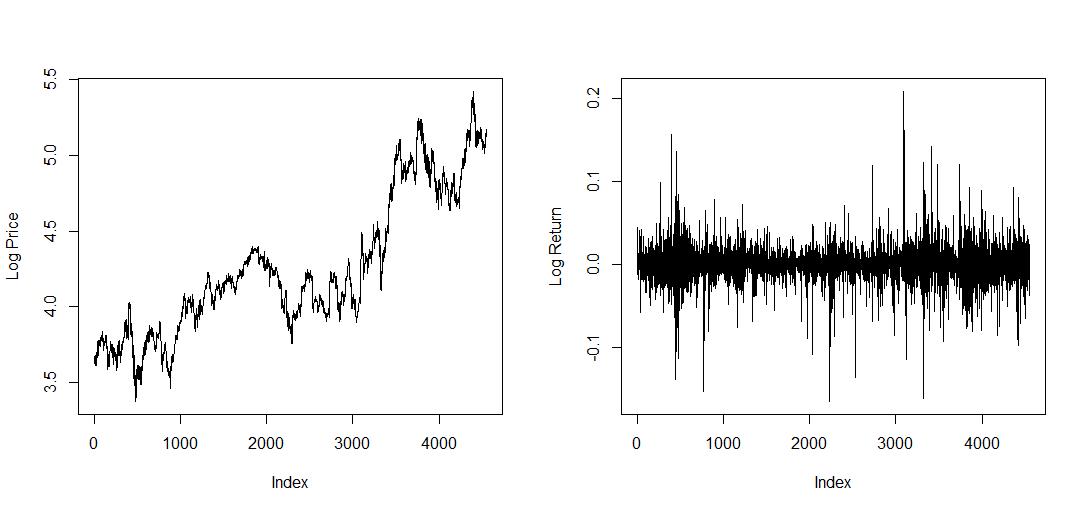
\includegraphics[width=0.9\linewidth]{plots/qcom_log_price_return.png}
	\caption{Time Series of QCOM Log Prices and Returns }
	\label{fig:qcom_log_price}
\end{figure}

Figure (\ref{fig:qcom_log_price}) shows the log returns and prices of the QCOM. We took the log transformation for two reasons. First, it is used to handle the exponential growth of the series, which the plot on the left confirms that the growth is linear on a log scale. Second, the transformation is used to stablize the variability of the series. With these adjustments in mind, we can see that the log price exhibit an upward trend. On the other hand, the variability changes throughout the time series when it comes to the log returns. Despite this, the log of the log returns is clearly stationary. We implemented the augmented Dickey-Fuller test on both the log prices and returns.
\begin{table}[ht]
	\centering
	\caption{Augmented Dick-Fuller Test for QCOM}
	\begin{tabular}[t]{lcccc}
		\toprule
		Time Series &Lag order& t-statistic & $p$-value & Outcome  \\
		\midrule
		Log Prices & 16 & -3.051 & 0.1333 & Unit-Root  \\				
		Log Returns & 16 & -16.254 & 0.01 & Stationary  \\				
		\bottomrule
	\end{tabular}\label{tab:adftest}
\end{table}
Table (\ref{tab:adftest}) shows the output of the augmented Dickey-Fuller test for the log prices and returns of QCOM. As we can see our suspicions were correct; we fail to reject the null-hypothesis for the log prices, but reject the null-hypothesis for the log returns. As such, the log returns are stationary, while the log prices exhibit unit-root.

We establish the time series' seasonality by examining the log prices' sample ACF. Figure (\ref{fig:qcom_acf_plots}) shows the ACF plots of QCOM with varying differencing and seasonality implementations. We have used a maximum lag of 100, with the time and seasonal differencing of once every 30 lags. The autocorrelation plot on the top right contains a very high and slow decay, starting from 1 at lag 0, which decreases gradually. This is typical of a non-stationary time series, where the values of the sample ACF are highly dependent on their past, such as a random walk.

\begin{figure}[h]
	\centering
	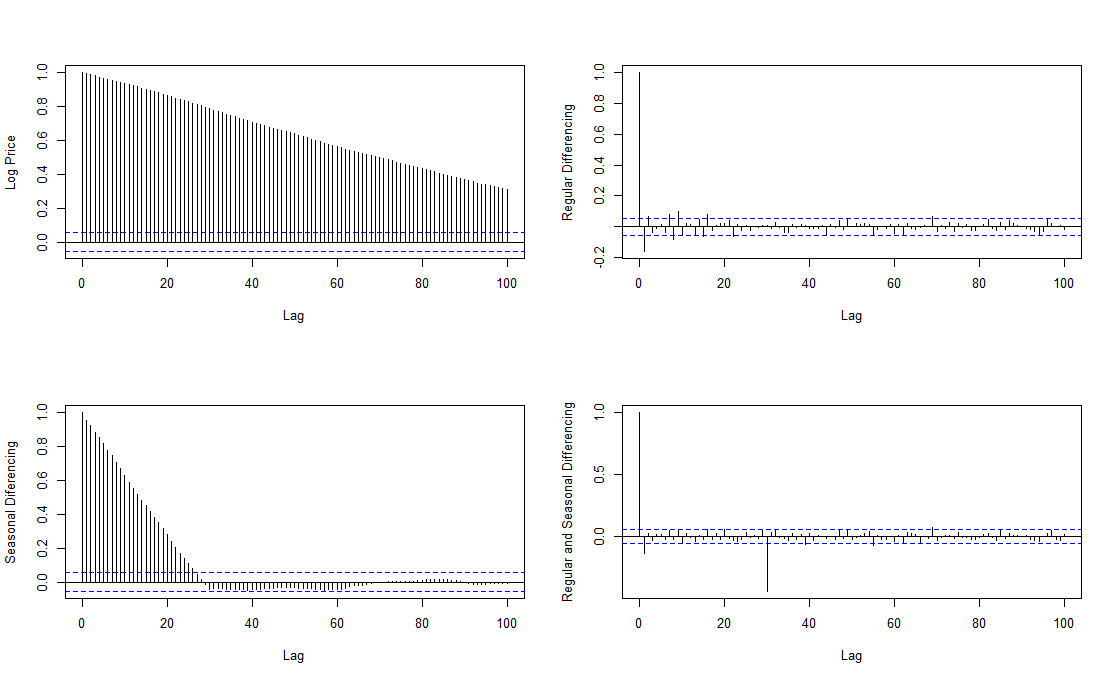
\includegraphics[width=1\linewidth]{plots/acf_plot_time_series.png}
	\caption{ACF Plot of QCOM }
	\label{fig:qcom_acf_plots}
\end{figure}

The plot on the top right shows the ACF of the First differenced log prices of the daily log prices. We can see a sharp drop in the autocorrelation at lag 1, where the other lags are within the confidence bounds. The first differencing has successfully removed the trend, producing a series that now looks more like white noise. 

On that bottom left plot, we have the ACF of the seasonal differencing, with a strong autocorrelation at lower lags, which slowly decreases to zero around lag 30. The differencing involves the following formula

\begin{equation}
	\Delta_{30}(\Delta x_t)=(1-B^{30})\Delta x_t=\Delta x_t-\Delta x_{t-30}
\end{equation}

After lag 30, the values fluctuate randomly around zero. This suggests that seasonal differencing alone removes the long-run periodicity but not the trend of the time series. In other words, seasonal differencing alone is not enough to transform the plot into a stationary time series.

The final plot on the bottom right shows the ACF after regular and seasonal differencing. The pattern shows that almost all autocorrelations are within the confidence bands, except for a substantial spike at lag one and lag 30, which suggest a seasonal lag. As we can see, combining regular and seasonal differencing yields a stationary series, and the residual autocorrelations are minimal. These transformations show that the plots on the bottom left and right show a stationary transformation. Fitting an ARIMA model would involve implementing either regular differencing or both regular and seasonal differencing.

\section*{ARIMA Model}

The goal of this section is to fit log prices and log returns into an autoregressive (AR), moving average (MA), or some combination of the two (ARMA, ARIMA). Figure (\ref{fig:acf_pacf_log_price_returns}) shows the ACF for the log prices (a), PACF of the log prices (b), ACF for the log returns (c) and the PACF for the log returns (d). For AR models, we would expect the ACF to show a gradual decay where the tail cuts off at some point, where the PACF would sharply cut off at lag $p$, then drop to approximately zero. We expect the opposite for MA models, where the ACF significantly cuts off at lag $q$ (then drops off to near zero), and the ACF gradually decays. On the other hand, the ACF and PACF for the ARMA(p,q) model will not clearly indicate where the lags cut off. 

\begin{figure}[h]
	\centering
	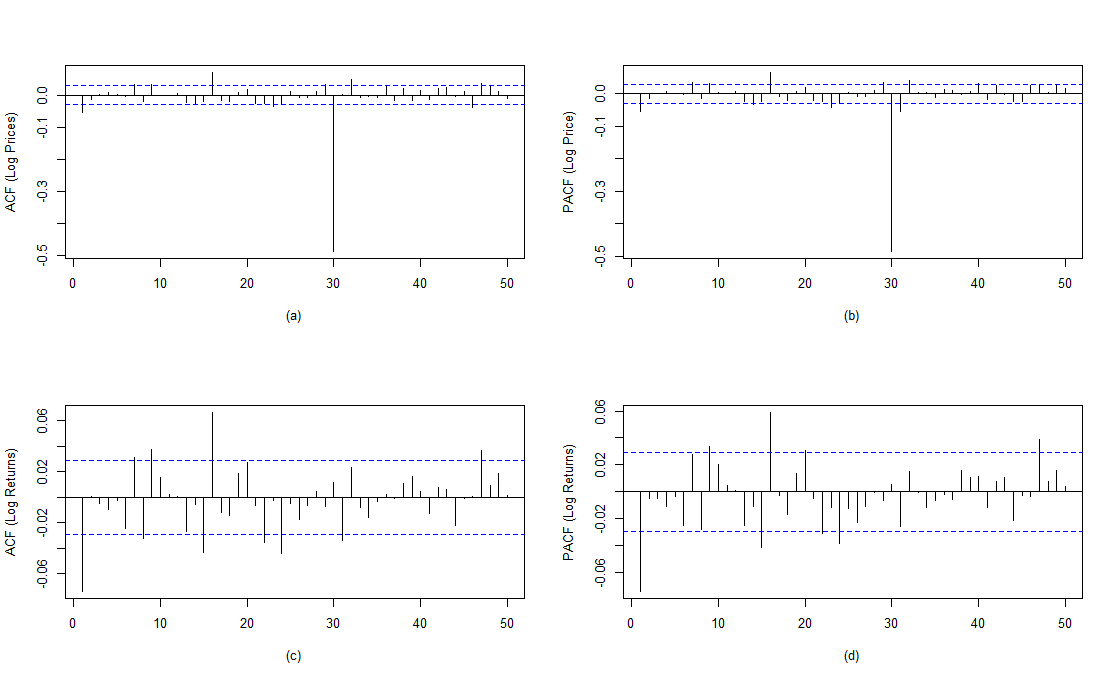
\includegraphics[width=1\linewidth]{plots/acf_pacf_log_price_returns.png}
	\caption{ACF and PACF for the log returns/prices of QCOM}
	\label{fig:acf_pacf_log_price_returns}
\end{figure}

We first examine the log prices of QCOM. As we can see from Figure (\ref{fig:acf_pacf_log_price_returns}), the ACF plot (a) for the log prices shows a very sharp spike at lag 0, and a significant lag around point 30; the rest is essentially noise. This plot is not very useful, because the time series is non-stationary. We have the same pattern when looking at the PACF plot (b) for the log prices, as we see mostly noise and a large spike around lag 30. Again, this plot is not very reliable since stationary is required for the PACF/ACF patterns to inform model selection. 

Looking at the ACF plot (c) log returns, we have a slight negative spike at lag 1. We also have a lot of significant lags that show up every 3 or 4 lags. Looking at the PACF plot (d), there are many small spikes, some of which are at lag 5, 8, 15, etc., but none are dominant. There is no clear cut-off in the PACF plot; we also do not see a gradual decline, which is consistent with the MA process. Using this plot, we cannot determine whether or not we should use an MA or AR model. We also consider using ARMA($p,q$) models.

The ARMA model (AutoRegression Moving Average) is a time series model used to describe stationary processes, which combines the past values of the AR($p$) model and the past forecasting errors of the MA($q$) model. We define the model as follows:
\begin{equation}
	r_t=\phi_0+\sum_{i=1}^{p}\phi_ir_{t-i}+a_t-\sum_{i=1}^{q}\theta_ia_{t-i},
\end{equation}
where $\lbrace a_t\rbrace$ is a white noise series and $p$ and $q$ are nonnegative integers. Since the ACF and PACF are not informative in determining the order of an ARMA model, we use the extended autocorrelation function (EACF) to specify the order of an ARMA process. If we have a consistent estimate of the AR component of an ARMA model, we can derive the MA component. From the derived MA series, we can use ACF to identify the order of an MA component.
\begin{table}[H]
	\centering
	\caption{Extended Autocorrelation Function (EACF) for QCOM Log Returns}
	\begin{tabular}{c|cccccccccccccc}
		$(p, q)$ & 0 & 1 & 2 & 3 & 4 & 5 & 6 & 7 & 8 & 9 & 10 & 11 & 12 & 13 \\
		\hline
		0 & x & o & o & o & o & x & x & x & x & o & o & o & o & o \\
		1 & x & o & o & o & o & o & o & o & o & o & o & o & o & o \\
		2 & x & o & o & o & o & o & o & o & o & o & o & o & o & o \\
		3 & x & o & o & o & o & o & o & o & o & o & o & o & o & o \\
		4 & x & x & o & o & o & o & o & o & o & o & o & o & o & o \\
		5 & x & x & x & o & o & o & o & o & o & o & o & o & o & o \\
		6 & x & x & x & x & o & o & o & o & o & o & o & o & o & o \\
		7 & x & x & x & x & x & o & o & o & o & o & o & o & o & o \\
		\label{tab:eacf}
	\end{tabular}
\end{table}
Unlike the standard ACF and PACF -- which are more effective for pure AR or MA models -- the EACF is especially useful when dealing with mixed ARMA models. The output of an EACF is a two-way table, where the rows correspond to AR order $p$ and the columns to MA order $q$. Table (\ref{tab:eacf}) shows the Theoretical EACF for an ARMA model, where X denotes statistically significant autocorrelation, and O denotes statistically insignificant autocorrelation, which suggests a good candidate for the true model. In general, for an ARMA($p,q$) model, the triangle of O will have its upper left vertex at the $(p, q)$ position, which we can see is an ARMA($1,1$) model. This will be the basis for our model selection.
\subsection*{Model Selection}

ARMA(1,1) is the basis for our models, but as we can see from the EACF, we can also consider entries that fall inside the "O triangle" (starting at $p=1,q=1$). The residuals at these points are also insignificant and potentially valid model candidates. Considering this, we also consider ARMA(1, 2), ARMA(2, 1), ARMA(2, 2), ARMA(1, 3), and ARMA(0, 2). We have picked a combination of models that either add an extra AR or MA term to balance our selection criteria. 

Table (\ref{tab:aic}) the selected fit for both the log returns and the log prices. The log prices includes both seasoning and regular differencing. For the selection criteria we use the AIC, which indicates a better-fitting model with a balance between the goodness of fit and model complexity. We choose the model with the smallest AIC, which is the ARMA(2,2) for the log prices and ARMA(0,2) for the log returns.

\begin{table}[ht]
	\centering
	\caption{AIC for Log Prices and Log Returns}
	\begin{tabular}[t]{lccccc}
		\toprule
		 			&ARMA(1,1)& ARMA(2,1) & ARMA(2,2) & ARMA(1,3) & ARMA(0,2)\\
		\midrule
		Log Prices & -21945.69 & -21943.79 & -21943.32 & -21941.81 & -21945.81  \\				
		Log Returns & -21958.18 & -21956.2 & -21954.39 & -21954.37 & -21958.15 \\				
		\bottomrule
	\end{tabular}\label{tab:aic}
\end{table}

\subsection*{Forecasting}

Like the behavior of ACF, forecast of an ARMA($p,q$) model have similiar characteristics as those of an AR($P$) model after adjusting for the impacts of the MA component. The form for the $\ell$-step-ahead forecast is the following:
\begin{equation}
	\hat{r}_h(\ell)=E(r_{h+\ell}|F_h)=\phi_0+\sum_{i=1}^{p}\phi_i\hat{r}_h(\ell-i)-\sum_{i=1}^{q}\theta_ia_h(\ell-i)
\end{equation}

Figure (\ref{fig:forecast}) presents a 1000-step ahead forecast for both the log prices (left panel) and log returns (right panel) of QCOM based on fitted ARIMA models.

The left panel shows the forecast from an ARIMA(2,1,2)(0,1,0) model applied to the log price series. The forecasted trajectory exhibits a flattening trend with widening confidence intervals over time, reflecting increasing uncertainty as the forecast horizon extends. Despite recent upward momentum in the log price, the model projects a relatively stationary mean path, suggesting that much of the recent trend may not persist in the long term. The fan-shaped prediction intervals highlight the stochastic nature of the process, primarily due to the seasonal and regular differencing applied.

\begin{figure}[h]
	\centering
	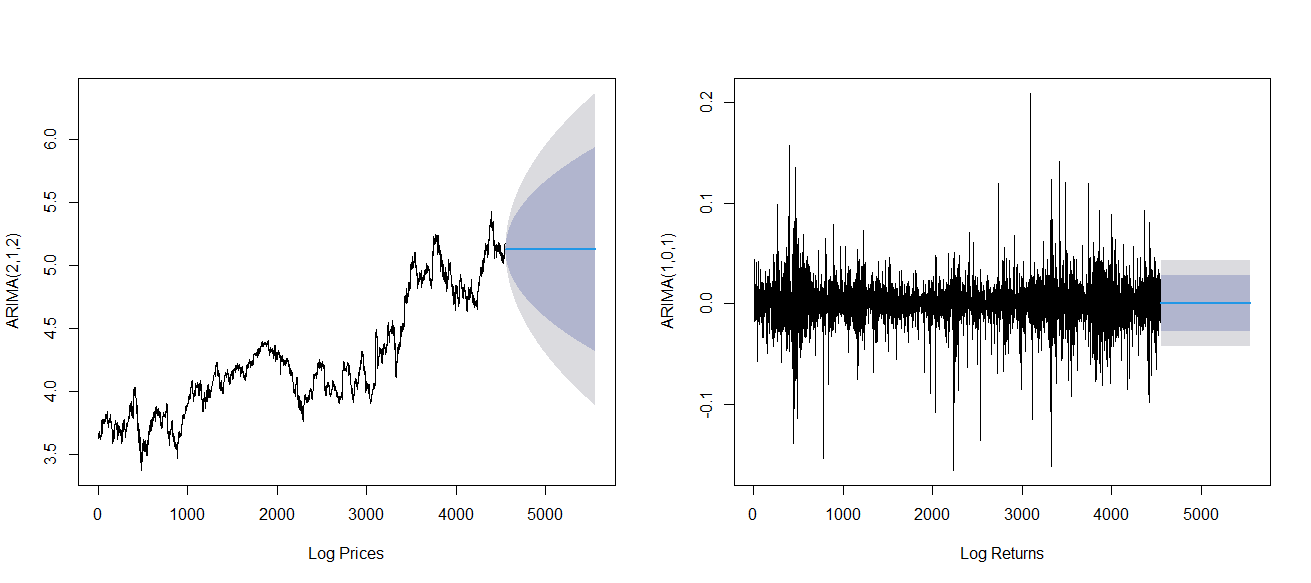
\includegraphics[width=1\linewidth]{plots/forecast.png}
	\caption{1000 Step Ahead Forecast for the Log Returns and Prices}
	\label{fig:forecast}
\end{figure}

Figure (\ref{fig:residual_plot_212}) shows the residual diagnostics for the fitted ARIMA(2,1,2) model applied to the QCOM log returns. The right panel displays the forecast from an ARIMA(0,1,1) model fitted to the log returns. The forecasted returns converge quickly to a mean close to zero, with narrow and stable confidence bands. This behavior aligns with the efficient market hypothesis, where log returns are assumed to be white noise, and thus, future returns are unpredictable based on past behavior. The low variance and flat mean reinforce the conclusion that the return process is stationary and lacks significant autocorrelation beyond short lags.

The right panel displays the forecast from an ARIMA(0,1,1) model fitted to the log returns. The forecasted returns converge quickly to a mean close to zero, with narrow and stable confidence bands. This behavior aligns with the efficient market hypothesis, where log returns are assumed to be white noise, and thus, future returns are unpredictable based on past behavior. The low variance and flat mean reinforce the conclusion that the return process is stationary and lacks significant autocorrelation beyond short lags.

Overall, the forecast results suggest that while log prices show medium-term variability and are influenced by both trend and seasonal components, the log returns remain largely mean-reverting with no significant drift, supporting the appropriateness of ARIMA models in modeling these two distinct dynamics.
\begin{figure}[h]
	\centering
	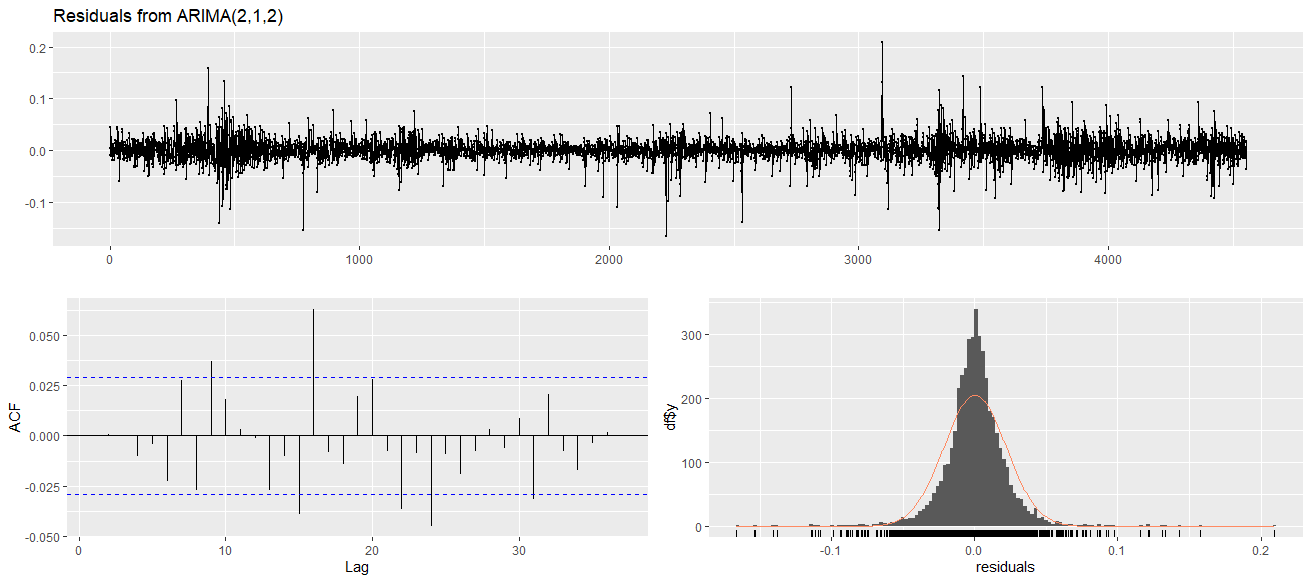
\includegraphics[width=1\linewidth]{plots/residual_plot_212.png}
	\caption{Residual Plots for the ARIMA(2,1,2) model for the Log Returns}
	\label{fig:residual_plot_212}
\end{figure}
The top panel shows the standardized residuals over time. The residuals appear to fluctuate around zero with no visible trend or systematic pattern, suggesting that the model has effectively captured the underlying structure of the time series. Some sporadic large residuals are observed, but they are infrequent and do not persist.

The bottom-left panel shows the ACF of the residuals, where most autocorrelations lie well within the 95\% confidence boundary. This indicates the absence of significant autocorrelation in the residuals, confirming that the ARIMA model has adequately removed time dependence from the series.

The bottom-right panel shows a histogram of the residuals overlaid with a normal density curve. The residuals are approximately centered at zero and exhibit a roughly bell-shaped distribution, although there is some evidence of slight fat tails compared to a normal distribution.

Overall, the diagnostic plots support the adequacy of the ARIMA(2,1,2) model. The residuals behave like white noise — they are uncorrelated and approximately normally distributed — suggesting that the model is a good fit for the data and suitable for forecasting purposes. Figure (\ref{fig:residual_plot_1_1}) also exhibits the same residual distribution for the ARIMA(1,0,1) model with the log prices.

\section*{Vector Autoregressive Models}

A Vector Autoregressive model of order $p$, denoted as $\text{VAR}(p)$, is used to model multivariate time series where each variable depends linearly on its own past values and those of other variables in the system. In contrast to univariate autoregressive models, VAR models account for the interdependencies among multiple time series by allowing each variable in the system to depend not only on its own past values but also on the past values of all other variables. This makes VAR particularly suitable for analyzing financial and economic systems where variables are often jointly determined, such as stock returns.

For $k-$dimensional time series $r_t$, the $\text{VAR}(p)$ model is specified as 
\begin{equation}
	r_t=\phi_0+\Phi_1 r_{t-1}+\cdots+\Phi_pr_{t-p}+a_t
\end{equation}
where $\Phi_0$ is a $k\times 1$ vector of constants, $\Phi_j$ is a $k\times k$ autoregressive coefficient matrix, and $a_t$ is a white noise innovation vector $\amsbb{E}[a_t]=0$ and $\text{Cov}(a_t)=\Sigma_a,$ a positive definite matrix.

One of the key strengths of VAR models is their ability to facilitate impulse response analysis, which tracks how a shock to one variable affects the entire system over time. This is useful in understanding transmission mechanisms, such as how a central bank interest rate change impacts inflation and output. Another common application is forecast error variance decomposition, which quantifies the contribution of each variable’s shock to the forecast error variance of others, offering insights into relative importance.

\begin{figure}[!h]
	\centering
	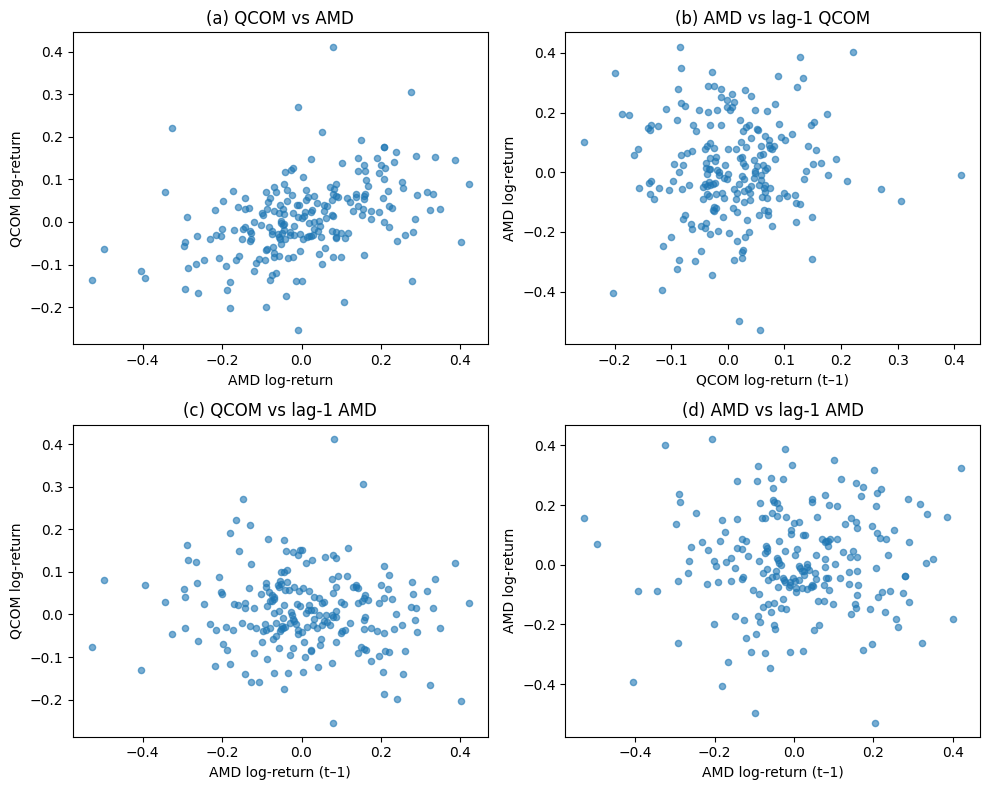
\includegraphics[width=0.8\linewidth]{plots/amd_qcom_scatter.png}
	\caption{Scatter Plot of Monthly log returns of AMD and QCOM}
	\label{fig:amd_qcom_scatter}
\end{figure}

Figure (\ref{fig:amd_qcom_scatter}) shows a panel of scatterplots, which illustrates the joint behavior and possible dynamic interactions between the monthly log returns of AMD and QCOM. In plot (a), which compares the concurrent log returns of QCOM and AMD, we observe a moderate positive association. This indicates that when AMD experiences a positive or negative return in a given month, QCOM tends to move in the same direction. This contemporaneous correlation suggests shared exposure to common market factors or industry-specific dynamics (both being semiconductor firms).

Plot (b) investigates whether QCOM’s past return (lag-1) helps explain AMD’s current return. The scatter shows weak structure and appears diffuse, suggesting limited predictive power from QCOM’s previous month return on AMD's current return. Likewise, plot (c) compares QCOM’s current return to AMD’s lag-1 return, and again, no strong relationship emerges, indicating that AMD’s past performance does not substantially inform QCOM’s present movement.

Finally, plot (d) looks at AMD's return against its own lag-1 value. The spread suggests minimal autocorrelation, which aligns with the empirical observation that individual stock returns are typically weakly autocorrelated at monthly frequencies due to market efficiency.

In our research, we we estimate a VAR(1) model using monthly log returns from QCOM (Qualcomm) and AMD (Advanced Micro Devices). The VAR(1) specification implies that each variable in the system is modeled as a linear function of one lag of both itself and the other variable, plus a constant and a random error term. This structure allows us to explore how past performance in one stock may influence future returns in both, offering insights into potential lead-lag relationships and co-movement dynamics in financial markets.

Matheamatically, a VAR(1) model for two variables can be expressed as the following:
\begin{equation}
	r_t=\phi_0+\Phi_{r_{t-1}}+a_t
\end{equation}

where $\phi_0$ is a $k-$dimensional vector, $\Phi$ is a $k\times k$ matrix, and $\lbrace a_t\rbrace$ is a sequence of serially uncorrelated random vectors with mean zero and covariance matrix $\Sigma$. The VAR(1) model consist of the following two equations:

\begin{equation}
\begin{aligned}
	r_{1t}=\phi_{10}+\Phi_{11}r_{1,t-1}+\Phi_{12}r_{2,t-1}+a_{1t},\\
	r_{2t}=\phi_{20}+\Phi_{21}r_{1,t-1}+\Phi_{22}r_{2,t-1}+a_{2t},\\
\end{aligned}
\end{equation}
The individual equations derived from the matrix form are QCOM returns:
\begin{equation}
\begin{aligned}
	\text{QCOM}_t=0.002356\cdot\text{QCOM}_{t-1}+0.03490\cdot\text{AMD}_{t-1}+2.1352\\
	\text{AMD}_t=-0.03611\cdot\text{QCOM}_{t-1}-0.08491\cdot\text{AMD}_{t-1}+1.9618\\
\end{aligned}
\end{equation}
which gives us the following matrix representation
\begin{equation}
	\begin{bmatrix}
		\text{QCOM}_t \\
		\text{AMD}_t
	\end{bmatrix}
	=
	\begin{bmatrix}
		2.1352 \\
		1.9618
	\end{bmatrix}
	+
	\begin{bmatrix}
		0.02356 & 0.03490 \\
		-0.03611 & -0.08491
	\end{bmatrix}
	\begin{bmatrix}
		\text{QCOM}_{t-1} \\
		\text{AMD}_{t-1}
	\end{bmatrix}
	+
	\begin{bmatrix}
		\epsilon_{\text{QCOM},t} \\
		\epsilon_{\text{AMD},t}
	\end{bmatrix}
\end{equation}
The QCOM equation shows weak positive autocorrelation and a mild positive effect from AMD’s previous return, suggesting slight predictive influence. The AMD equation exhibits negative coefficients for both lagged variables, indicating possible mean-reversion and a modest inverse relationship with QCOM’s past performance. The intercept terms represent average return levels adjusted for lagged influences.

Overall, the VAR(1) model captures the dynamic feedback between AMD and QCOM returns, allowing for richer modeling than univariate time series approaches. The small magnitude of the coefficients suggests that while interdependence exists, the direct predictive power is limited. However, even weak relationships can be valuable for short-term forecasting, constructing hedging strategies, or understanding market behavior under shocks (e.g., via impulse response functions). 

\section*{Cointegration}

In financial time series analysis, it is common to observe that individual asset prices or economic indicators follow nonstationary behavior, typically modeled as integrated processes of order one, \( I(1) \). However, economic theory often suggests that certain groups of such variables move together in the long run, maintaining stable equilibrium relationships despite short-term fluctuations. This phenomenon is known as \textit{cointegration}. Formally, if \( x_{1t} \) and \( x_{2t} \) are both \( I(1) \) series, they are cointegrated if there exists a scalar \( \gamma \) such that the linear combination \( w_t = x_{1t} - \gamma x_{2t} \) is stationary (\( I(0) \)). The vector \( (1, -\gamma) \) is then called the cointegrating vector, and \( w_t \) represents the equilibrium error or spread.

To formally test and model cointegrated systems, particularly in higher dimensions, the \textit{Vector Error Correction Model (VECM)} framework is employed. This begins by rewriting a VAR(\(p\)) model of nonstationary series \( X_t \) in terms of first differences, yielding the VECM:
\begin{equation}
	\Delta X_t = \Pi X_{t-1} + \sum_{i=1}^{p-1} \Phi_i^* \Delta X_{t-i} + a_t
\end{equation}
Here, the matrix \( \Pi = \Phi_1 + \cdots + \Phi_p - I \) captures the long-run relationships, while \( \Phi_i^* \) represent short-run dynamics. The key insight is that the rank of \( \Pi \) determines the cointegration structure: if \( \text{rank}(\Pi) = r < k \), then there exist \( r \) cointegrating vectors, and we can factor \( \Pi \) as \( \alpha \beta' \), where \( \beta \) contains the cointegrating vectors and \( \alpha \) reflects the speed of adjustment toward long-run equilibrium.

Cointegration has significant implications in financial applications. For instance, in \textit{pairs trading}, if two stock prices are cointegrated, the spread \( w_t = p_{1t} - \gamma p_{2t} \) will be mean-reverting, allowing traders to exploit deviations from the equilibrium for profit. A trading strategy might involve taking a long position in one stock and a short position in the other when the spread deviates from its historical mean by a certain threshold. 

The Johansen test, based on estimating the rank of \( \Pi \) in the VECM, is the standard method for identifying such cointegrating relationships in multivariate systems. The hypothesis test is as follows:
\begin{equation}
	\begin{aligned}
		&H_0:\text{rank}(\Pi)\leq r\\
		&H_a:\text{rank}(\Pi)>r
	\end{aligned}
\end{equation}
So increasing the assumed rank and testing how many stationary combinations exists. 

\begin{figure}[!h]
	\centering
	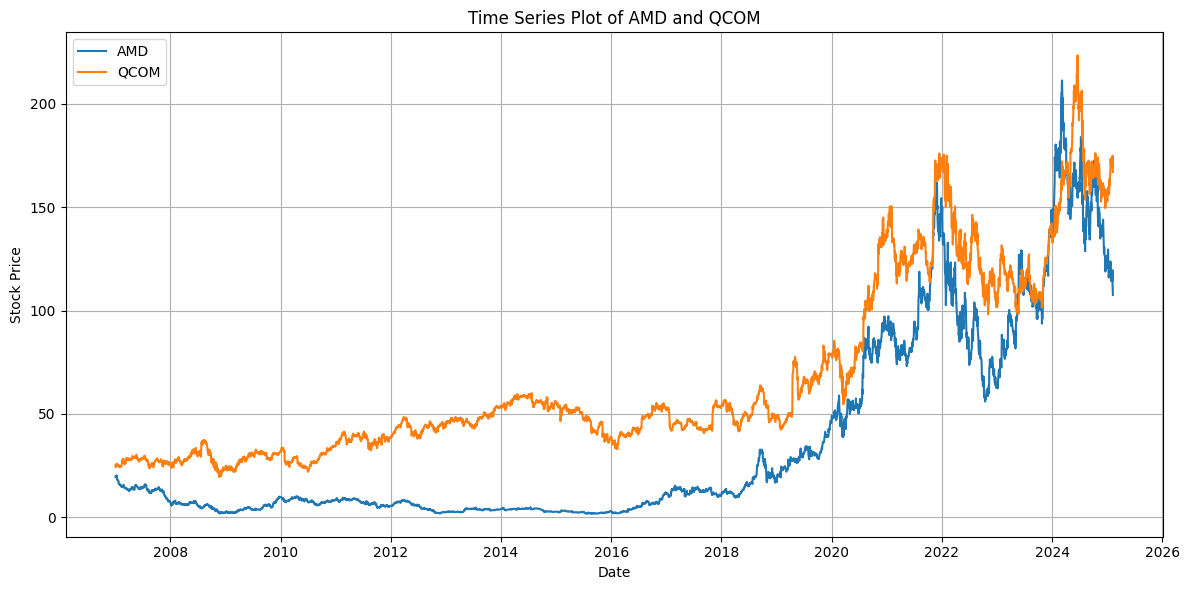
\includegraphics[width=0.8\linewidth]{plots/QCOM_AMD.png}
	\caption{Cumulative Returns of QCOM and AMD}
	\label{fig:amd_qcom_cumul_returns}
\end{figure}
Figure (\ref{fig:amd_qcom_cumul_returns}) shows the cumulative returns for both QCOM and AMD. The two series seem to trach each other, especially in the later half of the sample. This suggest that a stationary spread may exists ($\omega_t=\text{QCOM}_t-\gamma\cdot\text{AMD}_t$)

\newpage

\subsection*{NVDA Volatility Models}

This section presents a comparative analysis of two volatility models—ARCH(1) and GARCH(1,1) applied to the log returns of NVDA. The objective is to assess which model better captures the time-varying conditional heteroskedasticity in the return series, based on both statistical diagnostics and residual behavior.

\subsubsection*{ARCH(1) Models}


Despite the statistical significance of the estimated parameters, the ARCH(1) model failed to fully capture the volatility dynamics of the NVDA returns. The ACF and PACF plots of squared standardized residuals revealed strong autocorrelation at multiple lags, indicating the persistence of conditional heteroskedasticity in the residuals. This diagnosis is supported by the results of the Ljung-Box test on squared residuals, which returned a highly significant $p$-value ($p < 0.001$), leading to rejection of the null hypothesis of no autocorrelation.

\begin{figure}[!h]
	\centering
	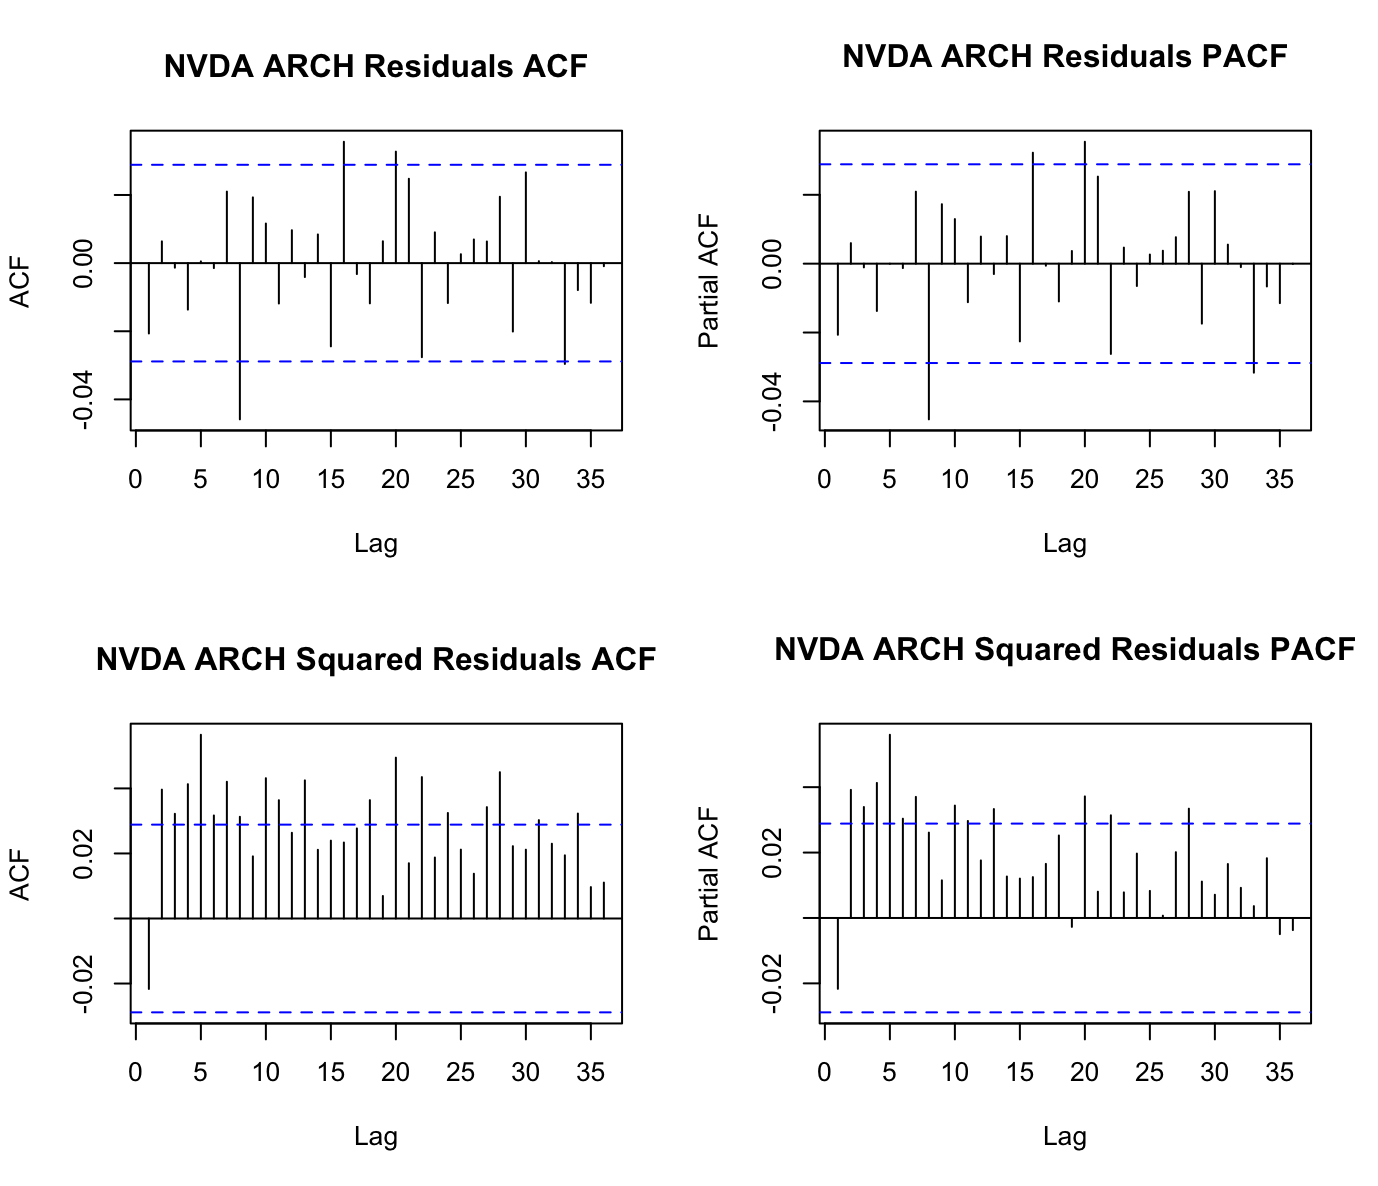
\includegraphics[width=0.8\linewidth]{plots/ARCH_NVDA.png}
	\caption{ACF and PACF of the Regular and Squared Residuals for NVDA ARCH Model}
	\label{fig:nvda_arch}
\end{figure}

Furthermore, the ARCH LM test statistics at lags 2, 4, and 6 all produced significant $p$-values (p < 0.01), confirming the presence of remaining ARCH effects. The Nyblom stability test reported joint and individual statistics that exceeded critical values, suggesting some parameter instability, particularly in the variance dynamics (omega and shape). Lastly, the Sign Bias test showed evidence of asymmetric effects (joint $p$-value = 0.0266), implying that positive and negative shocks affect volatility differently—something the ARCH model does not account for.

\subsubsection*{GARCH(1,1,)}

The GARCH(1,1) model (sGARCH(1,1)) was estimated using the same distributional assumptions and mean model. The parameter estimates for alpha1 and beta1 were highly significant, while the constant term (omega) was only marginally significant. The model achieved a higher log-likelihood value of 10177.79 and a lower AIC of -4.4114, indicating a better overall fit compared to the ARCH(1) model.

\begin{figure}[!h]
	\centering
	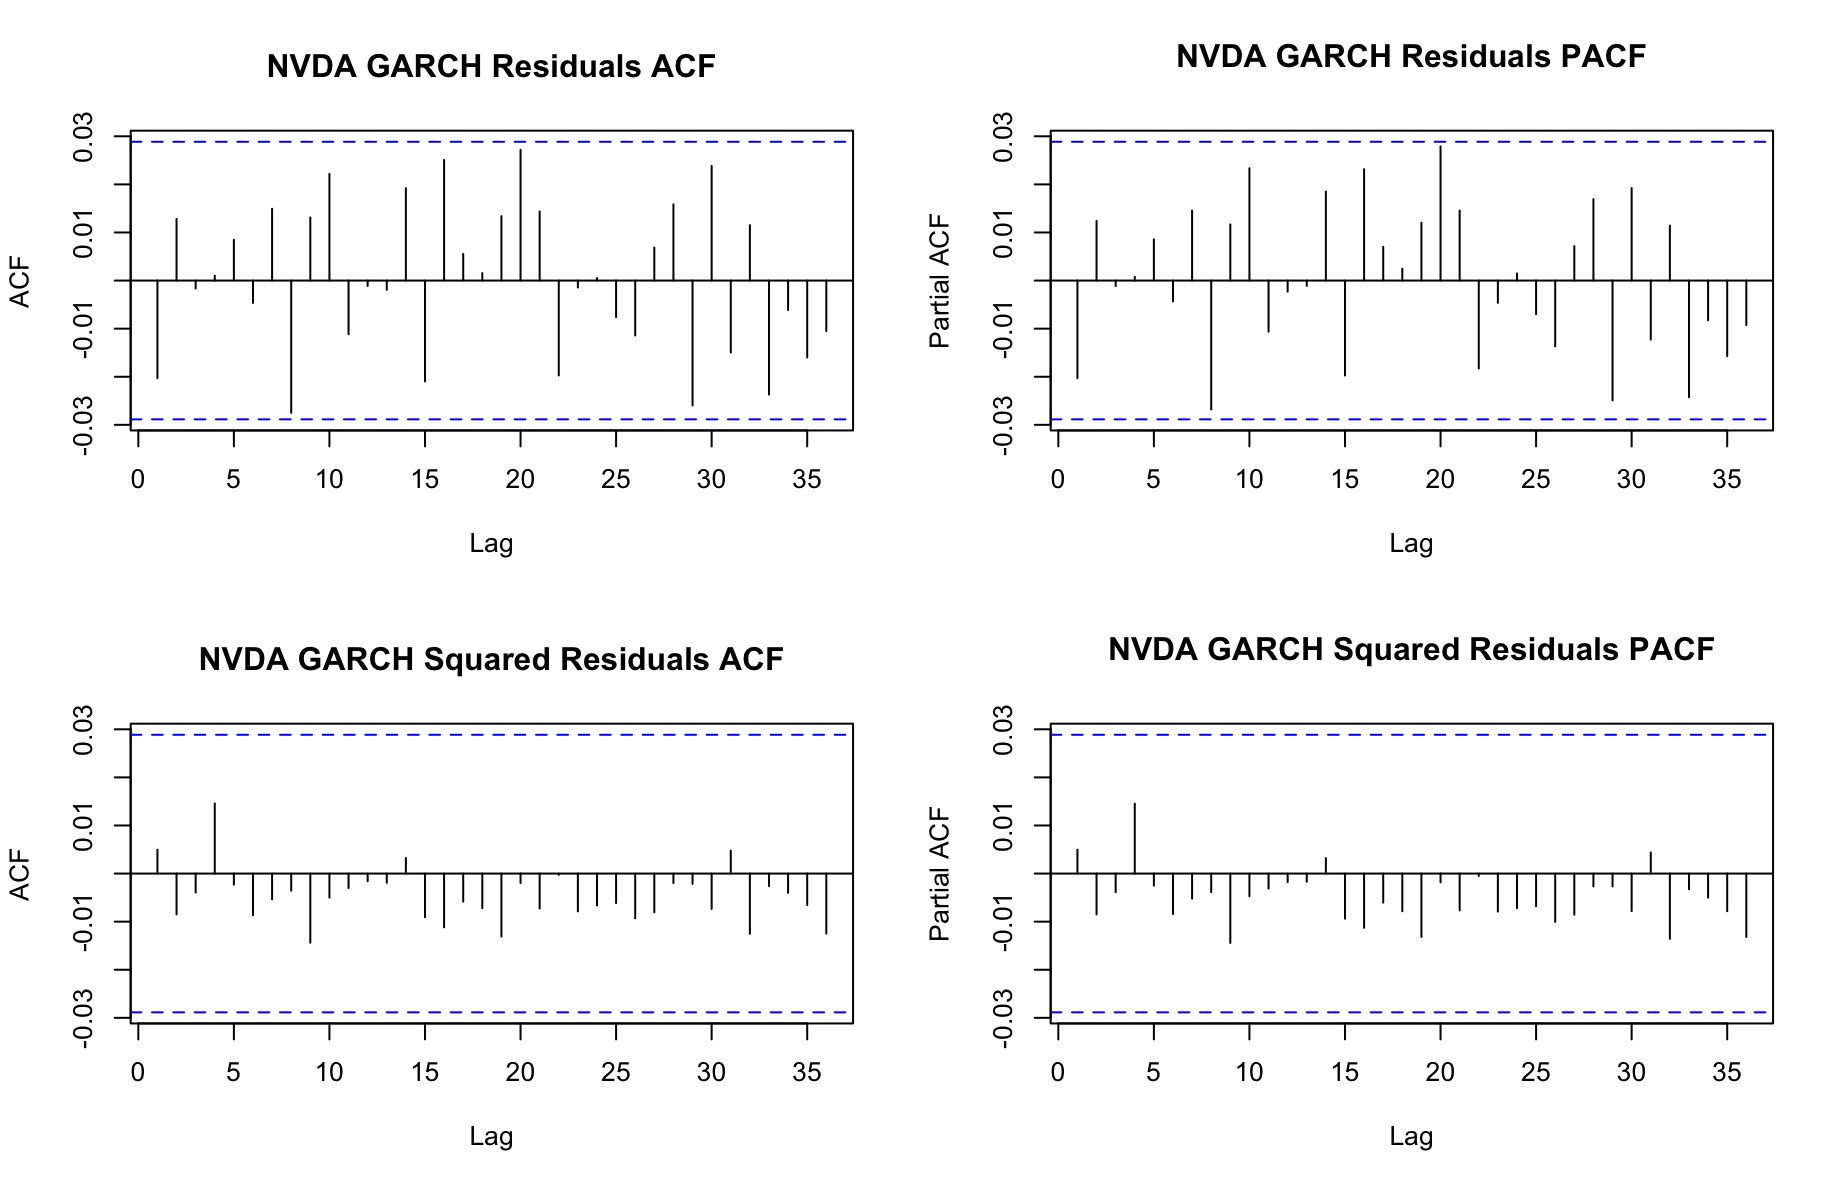
\includegraphics[width=0.8\linewidth]{plots/GARCH_NVDA.png}
	\caption{ACF and PACF of the Regular and Squared Residuals for NVDA GARCH Model}
	\label{fig:garch_nvda}
\end{figure}

Most notably, the ACF and PACF plots of squared standardized residuals under the GARCH model revealed minimal autocorrelation. The Ljung-Box test on squared residuals returned a p-value of 0.9782, strongly supporting the null hypothesis of no remaining autocorrelation. Similarly, the ARCH LM tests showed no significant ARCH effects at lags 3, 5, or 7 $(p > 0.75 )$, confirming that the GARCH(1,1) model adequately captures the time-varying volatility structure of NVDA returns.

\begin{table}[h!]
	\centering
	\caption{Weighted Ljung-Box Test Results for NVDA ARCH(1) and GARCH(1,1)}
	\begin{tabular}{llccc}
		\hline
		\textbf{Model} & \textbf{Residual Type} & \textbf{Lag} & \textbf{Statistic} & \textbf{p-value} \\
		\hline
		ARCH(1)   & Standardized Residuals      & Lag[1]              & 1.969   & 0.1606 \\
		&                             & Lag$(2(p+q)+(p+q)-1)$ & 2.063   & 0.2526 \\
		&                             & Lag$4((p+q)+(p+q)-1)$ & 2.468   & 0.5126 \\
		& Squared Residuals           & Lag$(1)$              & 2.166   & 0.1411 \\
		&                             & Lag$(2(p+q)+(p+q)-1)$ & 5.790   & 0.0250 \\
		&                             & Lag$(4(p+q)+(p+q)-1)$ & 16.934  & 0.0001 \\
		GARCH(1,1) & Standardized Residuals     & Lag[1]              & 1.905   & 0.1676 \\
		&                            & Lag$(2(p+q)+(p+q)-1)$ & 2.284   & 0.2197 \\
		&                            & Lag$(4(p+q)+(p+q)-1)$ & 2.587   & 0.4875 \\
		& Squared Residuals          & Lag$(1)$              & 0.114   & 0.7352 \\
		&                            & Lag$(2(p+q)+(p+q)-1)$ & 0.820   & 0.8989 \\
		&                            & Lag$(4(p+q)+(p+q)-1)$ & 1.450   & 0.9596 \\
		\hline
	\end{tabular}
	\label{tab:nvda_combined_wlb}
\end{table}

The results clearly demonstrate that the GARCH(1,1) model outperforms the ARCH(1) model in modeling NVDA return volatility. It provides better in-sample fit metrics, successfully eliminates residual autocorrelation in squared returns, and addresses conditional heteroskedasticity effectively. While both models exhibit some sign bias, indicating asymmetric volatility response, the overall diagnostics suggest that GARCH(1,1) is more appropriate for capturing volatility clustering in NVDA returns.

In summary, the GARCH(1,1) model should be preferred over the ARCH(1) model for financial modeling, risk management, and volatility forecasting tasks involving NVDA. However, the presence of asymmetry hints at further improvements using nonlinear or asymmetric volatility models, which are recommended for future exploration.

\subsection*{QCOM Volatility Models}

This section presents a comparative evaluation of ARCH(1) and GARCH(1,1) models fitted to the log returns of QCOM. We have the same objective as the NVDA time series.

\subsubsection*{ARCH(1)}

The ARCH(1) model is specified as a sGARCH(1,0) process under a zero-mean ARFIMA(0,0,0) structure and Student’s t-distributed innovations. All estimated parameters, including the mean ($\mu = 0.000735, \omega=0.000356, \text{ and } \alpha =0.4177$, and the shape parameter (3.2988), are statistically significant at the 1\% level under both standard and robust standard errors. The log-likelihood value achieved is 11768.02, and the AIC is -5.1015.

\begin{figure}[!h]
	\centering
	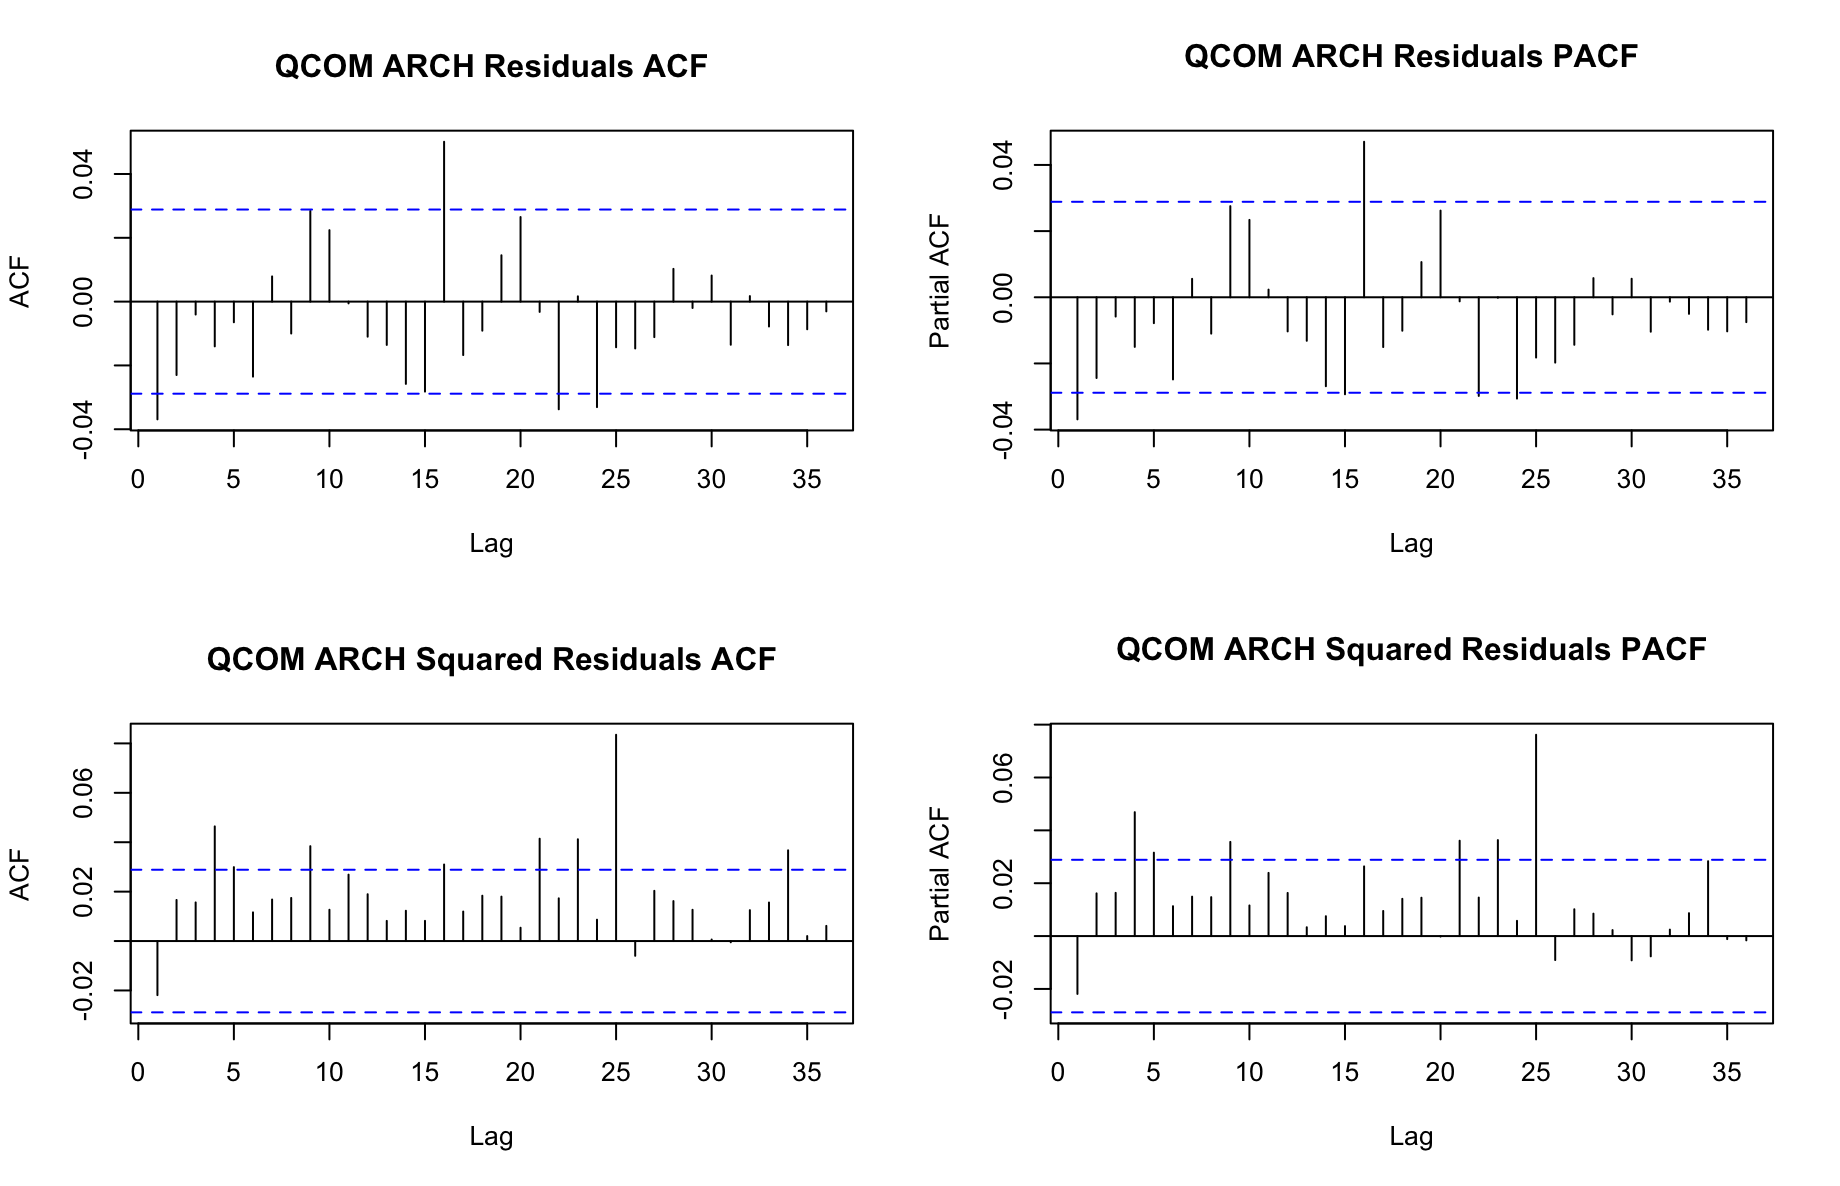
\includegraphics[width=0.8\linewidth]{plots/ARCH_QCOM.png}
	\caption{ACF and PACF of the Regular and Squared Residuals for QCOM ARCH Model}
	\label{fig:nvda_garch}
\end{figure}

Despite the strong parameter estimates, residual diagnostics suggest that the ARCH(1) model inadequately captures QCOM’s conditional heteroskedasticity. The ACF and PACF of the standardized residuals display persistent autocorrelation, especially at lags 1–20. The Ljung-Box test on residuals confirms this with a $p$-value of 0.037, indicating statistically significant autocorrelation.

Furthermore, the squared residuals’ ACF and PACF plots show moderate persistence across multiple lags. The Ljung-Box test on squared residuals has a $p$-value of 0.001, suggesting that residual volatility clustering remains. While the ARCH LM test is insignificant at lag 2 ($p$ = 0.26), it becomes significant at lags 4 and 6 ($p = 0.0269 \text{ and } 0.0074$), indicating remaining ARCH effects that the ARCH(1) model fails to capture.

\subsubsection*{GARCH(1,1)}

The GARCH(1,1) model builds upon the ARCH specification by introducing a lagged conditional variance term. Estimated parameters ($\mu = 0.000705, \omega = 0.000007, \alpha_1 = 0.0821, \beta = 0.9121$) are statistically significant, with the conditional variance showing high persistence ($\alpha + \beta \approx 0.994$). The model achieved a higher log-likelihood (11937.86) and a lower AIC of -5.1747, indicating a better fit than the ARCH(1) model.

The ACF and PACF plots both both standardized and squared standardized residuals show no significant autocorrelation. This is further supported by the Ljung-Box test results:

\begin{itemize}
	\item Standardize residuals: $p=0.373$
	\item Squared residual: $p=0.09932$
\end{itemize}

These results indicate that the GARCH(1,1) model effectively removes both linear and nonlinear dependence in the residuals. Moreover, ARCH LM tests at lags 3, 5, and 7 are all highly insignificant ($p > 0.81$), confirming that no residual ARCH effects remain. This demonstrates that the GARCH model has adequately captured the conditional variance structure.

\subsubsection*{Model Comparisons}

\begin{table}[h!]
	\centering
	\caption{Weighted Ljung-Box Test Results for QCOM ARCH(1) and GARCH(1,1)}
	\begin{tabular}{llccc}
		\hline
		\textbf{Model} & \textbf{Residual Type} & \textbf{Lag} & \textbf{Statistic} & \textbf{p-value} \\
		\hline
		ARCH$(1)$   & Standardized Residuals      & Lag$(1)$              & 6.284   & 0.0122 \\
		&                             & Lag$(2(p+q)+(p+q)-1)$ & 7.505   & 0.0088 \\
		&                             & Lag$(4(p+q)+(p+q)-1) $& 8.686   & 0.0199 \\
		& Squared Residuals           & Lag$(1)$              & 2.210   & 0.1371 \\
		&                             & Lag$(2(p+q)+(p+q)-1)$ & 2.849   & 0.1542 \\
		&                             & Lag$(4(p+q)+(p+q)-1)$ & 8.714   & 0.0195 \\
		GARCH$(1,1)$ & Standardized Residuals     & Lag$(1)$              & 0.237   & 0.6268 \\
		&                            & Lag$(2(p+q)+(p+q)-1)$ & 1.338   & 0.4006 \\
		&                            & Lag$(4(p+q)+(p+q)-1)$ & 2.569   & 0.4915 \\
		& Squared Residuals          & Lag$(1)$              & 0.104   & 0.7471 \\
		&                            & Lag$(2(p+q)+(p+q)-1)$ & 0.292   & 0.9845 \\
		&                            & Lag$(4(p+q)+(p+q)-1)$ & 0.877   & 0.9908 \\
		\hline
	\end{tabular}
	\label{tab:qcom_combined_wlb}
\end{table}

A comparative analysis of the ARCH(1) and GARCH(1,1) models applied to QCOM’s return series reveals that the GARCH(1,1) specification provides a superior statistical fit. This is evidenced by a higher log-likelihood and a lower Akaike Information Criterion (AIC). Additionally, residual diagnostics demonstrate that the GARCH model effectively eliminates autocorrelation in both the standardized and squared residuals, indicating a proper capture of volatility clustering. The model also passes the ARCH LM tests, confirming the absence of remaining ARCH effects. Nyblom stability tests further support the robustness of the GARCH(1,1) model, showing no significant instability in parameter estimates.

In contrast, the ARCH(1) model exhibits residual autocorrelation, suggesting inadequate modeling of volatility dynamics. It also shows signs of model misspecification and parameter instability. While sign bias tests show no significant asymmetry under either model, the GARCH(1,1) specification clearly outperforms in terms of overall model adequacy. As a result, the GARCH(1,1) model is the preferred choice for modeling QCOM return volatility. Given the lack of significant asymmetric effects, more complex specifications such as EGARCH or GJR-GARCH are not warranted in this context.

\section*{Appendix}
\begin{appendices}
\subsection*{Figures}
\begin{figure}[h]
	\centering
	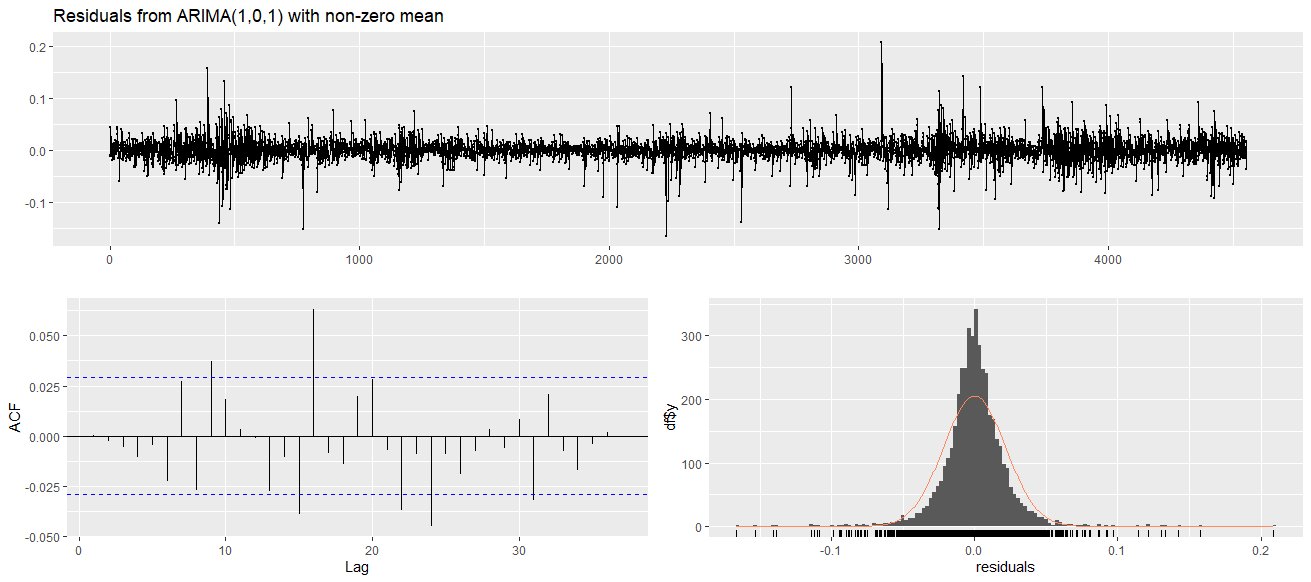
\includegraphics[width=1\linewidth]{plots/residual_plot_1_1.png}
	\caption{Residual Plots for the ARIMA(1,0,1) model for the Log Prices}
	\label{fig:residual_plot_1_1}
\end{figure}

\end{appendices}
\end{document}